\documentclass[12pt]{article}
\usepackage{mathtext} 
\usepackage{amsmath}

\usepackage[english, russian]{babel}
\usepackage[TS1, T2A]{fontenc}
\usepackage[utf8]{inputenc}
\usepackage{pscyr}

\usepackage[nomessages]{fp}
\usepackage{siunitx}
\sisetup{output-decimal-marker={,}}

\usepackage[left=2cm,right=2cm, top=1cm,bottom=1.5cm,bindingoffset=0cm]{geometry}

\usepackage{graphicx}
\graphicspath{{pictures/}}
\DeclareGraphicsExtensions{.pdf,.png,.jpg}

\begin{document}
	\pagestyle{empty}
	\begin{center}
		\normalsize
		\textbf{Федеральное государственное автономное образовательное учреждение высшего образования}

		\small
		\medskip 
		\textbf{САНКТ-ПЕТЕРБУРГСКИЙ НАЦИОНАЛЬНЫЙ ИССЛЕДОВАТЕЛЬСКИЙ  УНИВЕРСИТЕТ ИНФОРМАЦИОННЫХ ТЕХНОЛОГИЙ, МЕХАНИКИ И ОПТИКИ}

		\medskip 
		\textbf{ФАКУЛЬТЕТ ПРОГРАММНОЙ ИНЖЕНЕРИИ И КОМПЬЮТЕРНОЙ ТЕХНИКИ}
	\end{center}
	\bigskip\bigskip\bigskip\bigskip\bigskip\bigskip\bigskip\bigskip\bigskip\bigskip\bigskip\bigskip
	\begin{center}
		\par\medskip\par\smallskip
		\Large
 
		\par\smallskip
		\textbf{Основы электротехники} 

		\textbf{Домашняя работа №1}

		\large
		\par\bigskip
		\textbf{«Расчёт цепей постоянного тока»}
		\par\bigskip\par\bigskip\par\bigskip\par\bigskip\par\bigskip\par\bigskip
		\par\bigskip\par\bigskip\par\bigskip\par\bigskip\par\bigskip\par\bigskip
		\par\bigskip\par\bigskip\par\bigskip\par\bigskip\par\bigskip\par\bigskip
	\end{center}
	\begin{center}
		\begin{tabular}{lllll}
			Проверила:	 										& \hspace{80pt}	&	Выполнил:									&\\
			Никитина М.В	 \_\_\_\_\_\_\_\_\_\_\_\_\_\_		&				&	Студент группы P3255						&\\
			«\_\_\_\_\_\_» 	\_\_\_\_\_\_\_\_\_\_\_\_\_\_ 201\_г.& 				&	Федюкович С. А \_\_\_\_\_\_\_\_\_\_\_\_\_\_	&\\
																&				&	Вариант 12									&\\
																&				&												&\\
		\end{tabular}
		\par\bigskip\par\bigskip\par\bigskip
                                                  
		\par\bigskip \par\bigskip
	\end{center}
	\par\bigskip\par\bigskip\par\bigskip\par\bigskip\par\bigskip\par\bigskip\par\bigskip\par\bigskip
	\begin{center}
		Санкт-Петербург
		\par\bigskip
		2018
	\end{center}
	\newpage
	\pagestyle{plain}
	\setcounter{page}{1}
	\section*{Задание}
	\begin{center}
		{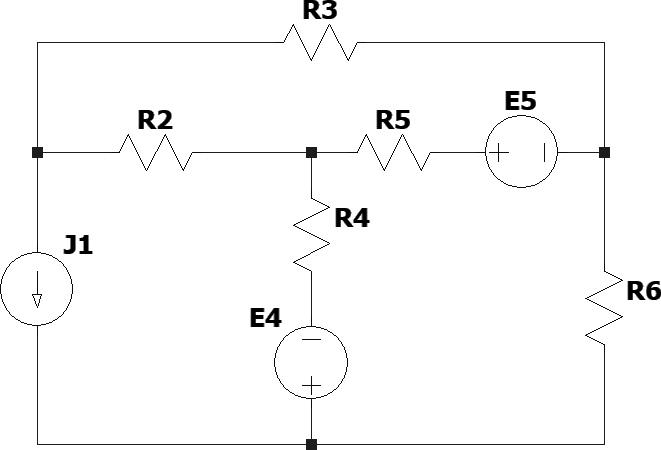
\includegraphics[scale=0.8]{1}}
	\end{center}
		
	\FPset{\eFour}{7} 	\FPset{\eFive}{24.5}
	\FPset{\rTwo}{1} 	\FPset{\rThree}{9} 		\FPset{\rFour}{4}
	\FPset{\rFive}{7}	\FPset{\rSix}{3} 		\FPset{\jOne}{0.3}	
	\textbf{Дано:}
	
	\par\bigskip
	 $E_4=\num{\eFour}[B]; E_5=\num{\eFive}[B];$ 	
	 
	 $R_2=\num{\rTwo}[Ом]; R_3=\num{\rThree}[Ом]; R_4=\num{\rFour}[Ом];$ 	
	 
	 $R_5=\num{\rFive}[Ом]; R_6=\num{\rSix}[Ом]; J_1=\num{\jOne}[A]$  			
	
	\par\bigskip
	\textbf{Найти:}

	\begin{enumerate}
		\item Значения всех неизвестных токов, используя законы Кирхгофа и метод контурных токов.
		\item Ток ветви $R_5$---$E_5$ методом эквивалентных преобразований.
		\item Напряжение, приложенное к источнику тока, мощность всех источников энергии, всех резистивных элементов, суммарную мощность источников цепи и суммарную мощность потребителей цепи.
	\end{enumerate}
		
	\section*{Решение}
	\subsection*{Задание 1}
	\subsubsection*{Решение через законы Кирхгофа}
		\begin{center}
			{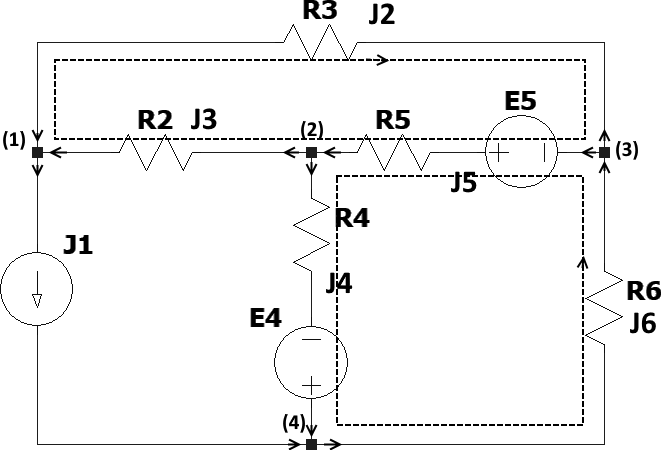
\includegraphics[scale=0.8]{2}}
			\par\bigskip
		\end{center}
		\begin{enumerate}
			\item Определим топологию цепи:	
					
			$p^*=6; p_{нт}=1; p=p^*-p_{нт}=6-1=5$		
				
			$g=4; n=p-(g-1)=5-(4-1)=2;$		
				
			$m_g=g-1=3; m_f=n=2$ 
			
			\item Система уравнений по законам Кирхгофа:
			
			 --- в общем виде: 
			
			$\begin{cases}
				J_2+J_3=J_1 						&\text{для узла (1)} 			\\
				J_5-J_3-J_4=0						&\text{для узла (2)} 			\\
				J_6-J_5-J_2=0						&\text{для узла (3)} 			\\
				R_6 J_6 + R_5 J_5 + R_4 J_4 = E_4 + E_5	&\text{для контура (3-2-4-3)}	\\	
				R_5 J_5 + R_2 J_3 - R_3 J_2= E_5		&\text{для контура (3-2-1-3)} 	\\
			\end{cases}$
			
			--- в матричной форме:
			
			\begin{tabular}{|ccccc|c|c|c|c|}
				$1$		&	$1$		&	$0$		& 	$0$		&	$0$		&		&	$J_2$	&		&	$J_1$		\\
				$0$		&	$-1$		&	$-1$		& 	$1$		&	$0$		&		&	$J_3$	&		&	$0$			\\
				$-1$		&	$0$		&	$0$		& 	$-1$		&	$1$		&	x	&	$J_4$	&	=	&	$0$			\\
				$0$		&	$0$		&	$R_4$	& 	$R_5$	&	$R_6$	&		&	$J_5$	&		&	$E_4+E_5$	\\
				$-R_3$	&	$R_2$	&	$0$		& 	$R_5$	&	$0$		&		&	$J_5$	&		&	$E_5$		\\
			\end{tabular}
			\newpage
			Подставив численные значения получаем: 
			
			\begin{tabular}{|ccccc|c|c|c|c|}
				$1$			&	$1$			&	$0$			& 	$0$				&	$0$			&		&	$J_2$	&		&	\num{\jOne}				\\
				$0$			&	$-1$			&	$-1$			& 	$1$				&	$0$			&		&	$J_3$	&		&	$0$						\\
				$-1$			&	$0$			&	$0$			& 	$-1$				&	$1$			&	x	&	$J_4$	&    $=$	&	$0$						\\
				$0$			&	$0$			&	\num{\rFour}	& 	\num{\rFive}		&	\num{\rSix}	&		&	$J_5$	&		&	\num{\eFour}$+$\num{\eFive}	\\
			  \num{-\rThree}	&	\num{\rTwo}	&	$0$			& 	\num{\rFive}		&	$0$			&		&	$J_5$	&		&	\num{\eFive}				\\		
			\end{tabular}
			
			\FPeval{\eFourFive}{round(eFour+eFive,1)}
			
			\begin{tabular}{|ccccc|c|c|c|c|}
				$1$			&	$1$			&	$0$			& 	$0$				&	$0$			&		&	$J_2$	&		&	\num{\jOne}				\\
				$0$			&	$-1$			&	$-1$			& 	$1$				&	$0$			&		&	$J_3$	&		&	$0$						\\
				$-1$			&	$0$			&	$0$			& 	$-1$				&	$1$			&	x	&	$J_4$	&    $=$	&	$0$						\\
				$0$			&	$0$			&	\num{\rFour}	& 	\num{\rFive}		&	\num{\rSix}	&		&	$J_5$	&		&	\num{\eFourFive}			\\
			  \num{-\rThree}	&	\num{\rTwo}	&	$0$			& 	\num{\rFive}		&	$0$			&		&	$J_5$	&		&	\num{\eFive}				\\		
			\end{tabular}
			
			\FPset{jTwo}{-0.58}
			\FPset{jThree}{0.88}
			\FPset{jFour}{1.74}
			\FPset{jFive}{2.62}
			\FPset{jSix}{2.04}
			\item Решая систему с помощью онлайн калькулятора, получаем: 
			
			\begin{tabular}{|c|c|c|c}
				$J_2$	&		&	\num{\jTwo}	&		\\
				$J_3$	&		&	\num{\jThree}	&		\\
				$J_4$	&   $=$	&	\num{\jFour}	&	,[А]	\\
				$J_5$	&		&	\num{\jFive}	&		\\
				$J_6$	&		&	\num{\jSix}	&		\\					
			\end{tabular}
		\end{enumerate}
		\subsubsection*{Решение методом контурных токов}
		\begin{center}
			{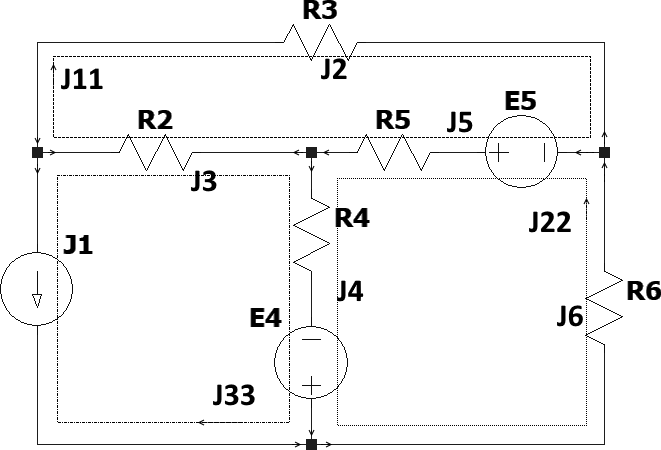
\includegraphics[scale=0.8]{3}}
			\par\bigskip
		\end{center}
		\FPeval{\jThreeThree}{round(-jOne,1)}
		\begin{enumerate}
			\item Выберем произвольно направления действительных токов $J_2-J_6;J_{33}=-J_1=\num{\jThreeThree}[А]$.
			\item Выделим два контура и укажем направления соответствующих токов.
			\item Определим собственные сопротивления токов:
			
			\FPeval{\rOneOne}{round(rThree+rTwo+rFive,0)}
			$R_{11}=R_3+R_2+R_5= \num{\rThree}+\num{\rTwo}+\num{\rFive}=\num{\rOneOne} [Ом]$
			
			\FPeval{\rTwoTwo}{round(rFour+rFive+rSix,0)}
			$R_{22}=R_4+R_5+R_6=\num{\rFour}+\num{\rFive}+\num{\rSix}=\num{\rTwoTwo} [Ом]$
			
			\item Определим общие сопротивления токов:
			
			\FPeval{\rOneTwo}{round(rFive,0)}
			$R_{12}=R_{21}=R_5=\num{\rOneTwo} [Ом]$
			
			\FPeval{\rOneThree}{round(-rTwo,0)}
			$R_{13}=-R_2=\num{\rOneThree} [Ом]$
			
			\FPeval{\rTwoThree}{round(rFour,0)}
			$R_{23}=R_4=\num{\rTwoThree} [Ом]$
			
			\item Определим собственные ЭДС токов:
			
			\FPeval{\eOneOne}{round(eFive,1)}
			$E_{11}=E_{5}=\num{\eOneOne} [В]$
			
			\FPeval{\eTwoTwo}{round(eFive+eFour,1)}
			$E_{22}=E_{5}+E_{4}=\num{\eFive}+\num{\eFour}=\num{\eTwoTwo} [В]$
			
			\item Составим и решим систему уравнений в общем виде: 
			
			$\begin{cases}
				R_{11}J_{11}+R_{12}J_{22}+R_{13}J_{33}=E_{11}	&	\text{для тока $J_{11}$} \\
				R_{21}J_{11}+R_{22}J_{22}+R_{23}J_{33}=E_{22}	&	\text{для тока $J_{22}$} \\
			\end{cases}$
			
			$\begin{cases}
				\num{\rOneOne} J_{11} + \num{\rOneTwo} J_{22} + (\num{\rOneThree}) \cdot (\num{\jThreeThree}) = \num{\eOneOne}	\\
				\num{\rOneTwo} J_{11} + \num{\rTwoTwo} J_{22} + \num{\rTwoThree} \cdot (\num{\jThreeThree}) = \num{\eTwoTwo}  	\\
			\end{cases}$
			
			\FPeval{\rjOneThree}{round(rOneThree*jThreeThree,1)}
			\FPeval{\rjTwoThree}{round(rTwoThree*jThreeThree,1)}
			$\begin{cases}
				\num{\rOneOne} J_{11} + \num{\rOneTwo} J_{22} + \num{\rjOneThree} = \num{\eOneOne}	\\
				\num{\rOneTwo} J_{11} + \num{\rTwoTwo} J_{22} \num{\rjTwoThree}= \num{\eTwoTwo}  	\\
			\end{cases}$
			
			\FPeval{\eOneOne}{round(eOneOne - rjOneThree,1)}
			\FPeval{\eTwoTwo}{round(eTwoTwo - rjTwoThree,1)}
			$\begin{cases}
				\num{\rOneOne} J_{11} + \num{\rOneTwo} J_{22} = \num{\eOneOne}		\\
				\num{\rOneTwo} J_{11} + \num{\rTwoTwo} J_{22} = \num{\eTwoTwo}  	\\
			\end{cases}$
			
			\item Решая систему с помощью онлайн калькулятора, получаем: 
			
			\FPeval{\jOneOne}{0.58}
			\FPeval{\jTwoTwo}{2.04}
			$\begin{cases}
				J_{11}=\num{\jOneOne}[A]	\\
				J_{22}=\num{\jTwoTwo}[A]	\\
			\end{cases}$
			
			\item Определим исходные токи:
			
			\FPeval{\jTwo}{round(-jOneOne,2)}
			$J_2 = -J_{11} = \num{\jTwo}[A];$
			
			\FPeval{\jThree}{round(jOneOne-jThreeThree,2)}
			$J_3 = J_{11}-J_{33} =\num{\jOneOne}-(\num{\jThreeThree}) = \num{\jThree}[A];$
			
			\FPeval{\jFour}{round(jTwoTwo+jThreeThree,2)}
			$J_4 = J_{22}+J_{33} =\num{\jTwoTwo}+(\num{\jThreeThree}) =\num{\jFour}[A];$
			
			\FPeval{\jFive}{round(jOneOne+jTwoTwo,2)}
			$J_5 = J_{11}+J_{22} =\num{\jOneOne}+\num{\jTwoTwo}= \num{\jFive}[A].$

			\FPeval{\jSix}{round(jTwoTwo,2)}
			$J_6 = J_{22}= \num{\jSix}[A];$
			
			\textbf{Ответ:} $J_2 = \num{\jTwo} [A]; J_3 = \num{\jThree} [A]; J_4 = \num{\jFour} [A]; J_5 = \num{\jFive} [A]; J_6 = \num{\jSix} [A].$
		\end{enumerate}
		\newpage
		\section*{Задание 2}
		\begin{enumerate}
			\item $J_1$ расцепляем на контур $R_6$---$R_3$:
			
			\FPeval{\jOneOne}{jOne}
			\FPeval{\jOneTwo}{jOne}
			$J_{11} = J_{12} = J_1 = \num{\jOne} [A]$
			\begin{center}
				{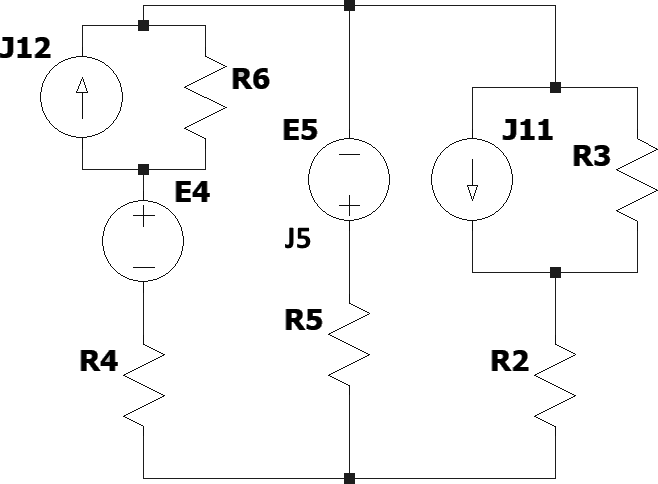
\includegraphics[scale=0.8]{4}}
				\par\bigskip
			\end{center}
			
			\item $J_{11} || R_3 \rightarrow E_3$---$R_3; J_{12} || R_6 \rightarrow E_6$---$R_6$;
			
			\FPeval{\eThree}{round(jOneOne*rThree,1)}
			$E_3=J_{11}\cdot R_3=\num{\jOneOne}\cdot \num{\rThree} = \num{\eThree}[B];$
			
			\FPeval{\eSix}{round(jOneTwo*rSix,1)}
			$E_6=J_{12}\cdot R_6=\num{\jOneTwo}\cdot \num{\rSix} = \num{\eSix}[B]$
			\begin{center}
				{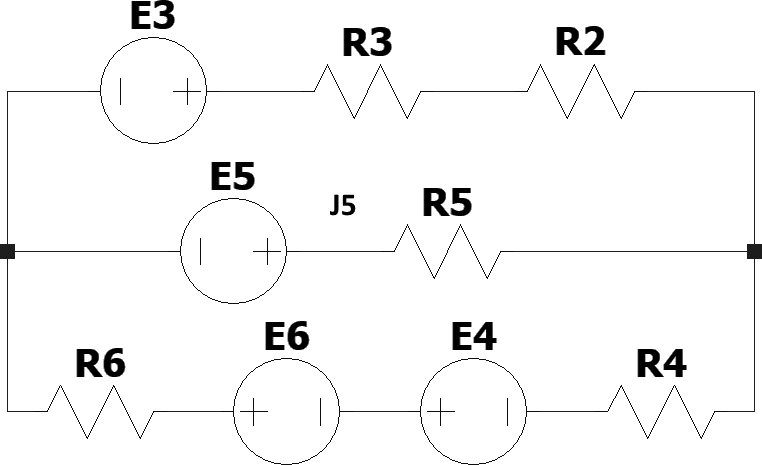
\includegraphics[scale=0.8]{5}}
				\par\bigskip
			\end{center}
			
			\item $(R_6,E_6,E_4,R_4)||(E_3,R_3,R_2)\rightarrow E_o, R_o$
			
			\FPeval{\rO}{round(((rSix+rFour)*(rThree+rTwo)/(rThree+rTwo+rSix+rFour)),2)}
			$R_o = \frac{(R_6+R_4) \cdot (R_3+R_2)}{R_6+R_4+R_3+R_2}=\frac{(\num{\rSix}+\num{\rFour}) \cdot (\num{\rThree}+\num{\rTwo})}{\num{\rSix}+\num{\rFour}+\num{\rThree}+\num{\rTwo}}=\num{\rO}[Ом]$
			
			\FPeval{\eO}{round( ( (eSix + eFour)/(rSix+rFour) + eThree/(rThree+rTwo))/(1/(rSix+rFour)+1/(rThree+rTwo)),2)}
			$E_o = \frac{(E_6+E_4)/(R_6+R_4) + E_3/(R_3+R_2)}{1/(R_6+R_4)+1/(R_3+R_2)} = \frac{(\num{\eSix}+\num{\eFour})/(\num{\rSix}+\num{\rFour}) + \num{\eThree}/(\num{\rThree}+\num{\rTwo})}{1/(\num{\rSix}+\num{\rFour})+1/(\num{\rThree}+\num{\rTwo})} = \num{\eO}[B]$
			\begin{center}
				{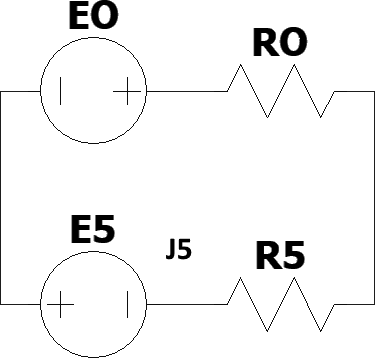
\includegraphics[scale=0.8]{6}}
				\par\bigskip
			\end{center}
			
			\item По второму закону Кирхгофа: 
			
			$J_5(R_o+R_5)=E_5 + E_o$
			
			$J_5=\frac{E_5 + E_o}{R_o+R_5}=\frac{\num{\eFive}+\num{\eO}}{\num{\rO}+\num{\rFive}}=2,62[А]$
			
			\textbf{Ответ:} $J_5 = 2,62[A].$
		\end{enumerate}
		
		\newpage
		\section*{Задание 3}
		\begin{center}
			{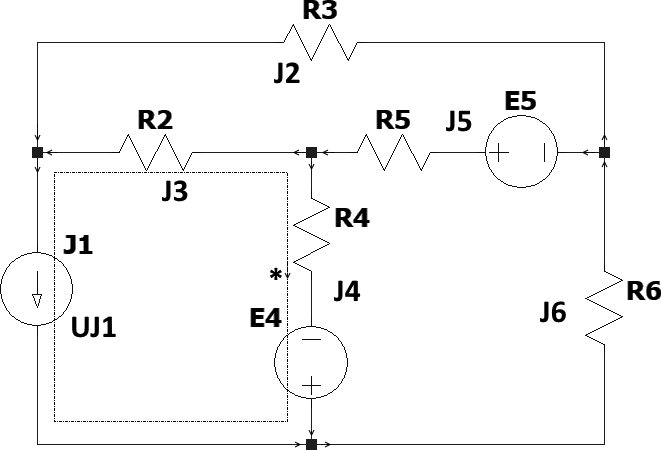
\includegraphics[scale=0.8]{7}}
			\par\bigskip
		\end{center}
		
		\begin{enumerate}
			\FPset{jTwo}{-0.58}
			\FPset{jThree}{0.88}
			\FPset{jFour}{1.74}
			\FPset{jFive}{2.62}
			\FPset{jSix}{2.04}
		
			\item Определим $U_{J1}$ по второму закону Кирхгофа для контура $(*)$:
			
			$-U_{J1}+R_4 J_4 - R_2 J_2=E_4$
			
			\FPeval{\uJ}{round(-(eFour+rTwo*jThree-rFour*jFour),2)}
			$U_{J1}=-E_4 - R_2 J_3+R_4 J_4=\num{\eFour} -\num{\rTwo}\cdot\num{\jThree}+\num{\rFour}\cdot \num{\jFour}=\num{\uJ}[B]$
			
			\item Определим мощности источников: 
			
			\FPeval{\pjOne}{round(-uJ*jOne,2)}
			$P_{J1}= -U_{J1} J_1 = -(\num{\uJ})\cdot \num{\jOne} = \num{\pjOne} [Вт]$
			
			\FPeval{\peFour}{round(eFour*jFour,2)}
			$P_{E4}= E_{4} J_4 = \num{\eFour}\cdot \num{\jFour} = \num{\peFour} [Вт]$
			
			\FPeval{\peFive}{round(eFive*jFive,2)}
			$P_{E5}= E_{5} J_5 = \num{\eFive}\cdot \num{\jFive} = \num{\peFive} [Вт]$
			
			\item Определим мощности резистивных элементов: 
			
			\FPeval{\prTwo}{round(rTwo*jThree*jThree,2)}
			$P_{R2}= R_{2} {J_3}^2 = \num{\rTwo}\cdot {\num{\jThree}}^2 = \num{\prTwo} [Вт]$
			
			\FPeval{\prThree}{round(rThree*jTwo*jTwo,2)}
			$P_{R3}= R_{3} {J_2}^2 = \num{\rThree}\cdot {(\num{\jTwo})}^2 = \num{\prThree} [Вт]$
			
			\FPeval{\prFour}{round(rFour*jFour*jFour,2)}
			$P_{R4}= R_{4} {J_4}^2 = \num{\rFour}\cdot {\num{\jFour}}^2 = \num{\prFour} [Вт]$
			
			\FPeval{\prFive}{round(rFive*jFive*jFive,2)}
			$P_{R5}= R_{5} {J_5}^2 = \num{\rFive}\cdot {\num{\jFive}}^2 = \num{\prFive} [Вт]$
			
			\FPeval{\prSix}{round(rSix*jSix*jSix,2)}
			$P_{R6}= R_{6} {J_6}^2 = \num{\rSix}\cdot {\num{\jSix}}^2 = \num{\prSix} [Вт]$
			
			\item Определим суммарные мощности: 
			
			\FPeval{\pis}{round(pjOne + peFour + peFive,2)}
			$P_и=P_{J1}+P_{E4}+P_{E5}= \num{\pjOne}+\num{\peFour}+\num{\peFive}=\num{\pis}[Вт]$
			
			\FPeval{\pirs}{round(prTwo + prThree + prFour + prFive + prSix,2)}
			$P_р=P_{R2}+P_{R3}+P_{R4}+P_{R5}+P_{R6}= \num{\prTwo}+\num{\prThree}+\num{\prFour}+\num{\prFive}+\num{\prSix}=\num{\pirs}[Вт]$
			
			\textbf{Ответ:}
			
			$U_{J1}=\num{\uJ}[B]; P_{J1}= \num{\pjOne} [Вт];P_{E4} = \num{\peFour} [Вт];P_{E5}= \num{\peFive} [Вт]$
			
			$P_{R2} = \num{\prTwo} [Вт];P_{R3}= \num{\prThree} [Вт];P_{R4}= \num{\prFour} [Вт];P_{R5}= \num{\prFive} [Вт];P_{R6}= \num{\prSix} [Вт]$
			
			$P_и=\num{\pis}[Вт];P_р=\num{\pirs}[Вт]$
			
		\end{enumerate}
\end{document}